\documentclass[hyperref={pdfpagelabels=false},usepdftitle=false]{beamer}
\usepackage{../templates/myStyle}

\begin{document}
\selectlanguage{english}

\title{\titleText}
\subtitle{Bachelor's thesis of Martin Thoma}
\author{\tutor}
\date{5th of June, 2014}
%\subject{Programmieren}

\frame{\titlepage}

\frame{
    \frametitle{Contents}
    \setcounter{tocdepth}{1}
    \tableofcontents
    \setcounter{tocdepth}{2}
}

%\AtBeginSection[]{
%    \InsertToC[sections={\thesection}]  % shows only subsubsections of one subsection
%}

\section{What is my Bachelor's thesis about?}
\chapter*{Introduction}
When you want to develop a selfdriving car, you have to plan which path 
it should take. A reasonable choice for the representation of
paths are cubic splines. You also have to be able to calculate
how to steer to get or to remain on a path. A way to do this
is by applying the \href{https://en.wikipedia.org/wiki/PID_algorithm}{PID algorithm}.
This algorithm needs to know the signed current error. So you need to 
be able to get the minimal distance of a point (the position of the car)
to a cubic spline (the prefered path)
combined with sign (which represents the steering direction).
As one steering direction might be prefered, it is not only necessary to
get the minimal absolute distance, but might also help to get all points
on the spline with minimal distance.

In this paper, I want to discuss how to find all points on a cubic 
function with minimal distance to a given point.
As other representations of paths might be easier to understand and
to implement, I will also cover the problem of finding the minimal
distance of a point to a polynomial of degree 0, 1 and 2.

While I analyzed this problem, I've got interested in variations
of the underlying PID-related problem. So I will try to give
robust and easy-to-implement algorithms to calculate the distance
of a point to a (piecewise or global) defined polynomial function
of degree $\leq 3$.

When you're able to calculate the distance to a polynomial which is
defined on a closed invervall, you can calculate the distance from
a point to a spline by calculating the distance to the pieces of the
spline.


\section{write-math.com}
\subsection{Write Math}

\begin{frame}{write-math.com}
    \begin{itemize}
        \item a website where users can add labeled training data
        \item works with desktop computers and touch devices
        \item symbol recognition can be done by multiple classifiers
        \item users can contribute formulas
        \item users can vote for formulas
        \item user who wrote the formula can accept one formula
    \end{itemize}
\end{frame}

\framedgraphic{Classify}{../images/classify.png}
\framedgraphic{Workflow}{../images/workflow.png}
% \framedgraphic{User page}{../images/user-page.png}
% \framedgraphic{Information about recordings}{../images/view.png}
% \framedgraphic{Symbol page}{../images/symbol.png}
% \framedgraphic{Training}{../images/train.png}
\framedgraphic{Ranking}{../images/ranking.png}


\begin{frame}[fragile]{Statistics}
    \begin{itemize}
        \item 127 users with at least 5 recordings
        \item 1109 symbols, but only 369 used for experiments
        \item $\num{235831}$ recordings (e.g. $\num{3486}$ times \verb+\int+)
    \end{itemize}
\end{frame}

\begin{frame}{First classification worker}
    \begin{itemize}
        \item preprocessing: Scale to fit into unit square while keeping the aspect
              ratio
        \item applies dynamic time warping
        \item compares a new recording with every recording
              in the database
        \item[$\Rightarrow$] Classification time is in $\mathcal{O}(\text{recordings})$,
              but we rather would like $\mathcal{O}(\text{symbols})$
        \item the current server / workflow can only handle about 4000 recordings
        \item[$\Rightarrow$] Another way to classify is necessary
    \end{itemize}
\end{frame}

\section{Preprocessing and Features}
\subsection{Preprocessing Algorithms}
\begin{frame}{Preprocessing Algorithms}
    \begin{columns}[T] % contents are top vertically aligned
    \begin{column}[T]{5cm} % each column can also be its own environment
        \begin{itemize}
            \item<1-> Normalizing
            \begin{itemize}
                \item<2-> Scaling
                \item<2-> Shifting
                \item<3-> Resampling
            \end{itemize}
            \item<1-> Noise reduction
            \begin{itemize}
                \item<4-> Smoothing (e.g. moving average)
                \item<5-> Dot reduction
                \item<6-> Filtering (by distance, speed or angle)
                \item<8-> Stroke connection
            \end{itemize}
        \end{itemize}
    \end{column}
    \begin{column}[T]{6cm} % alternative top-align that's better for graphics
        \only<2>{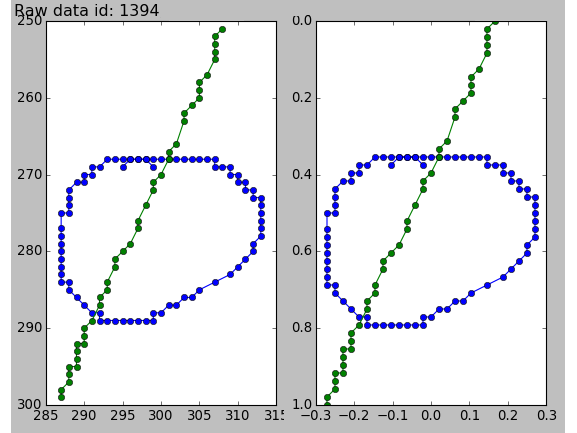
\includegraphics[width=6cm, keepaspectratio]{scale-and-shift.png}}
        \only<3>{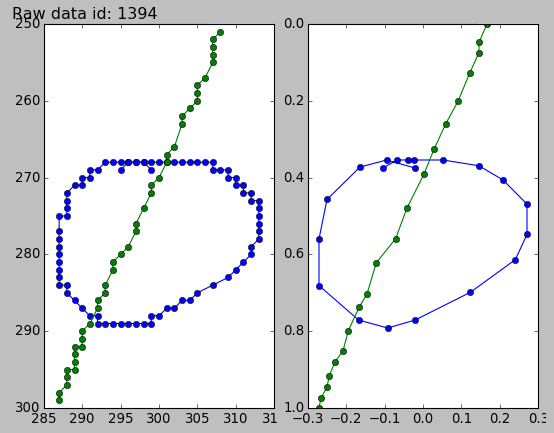
\includegraphics[width=6cm, keepaspectratio]{resampling.png}}
        \only<4>{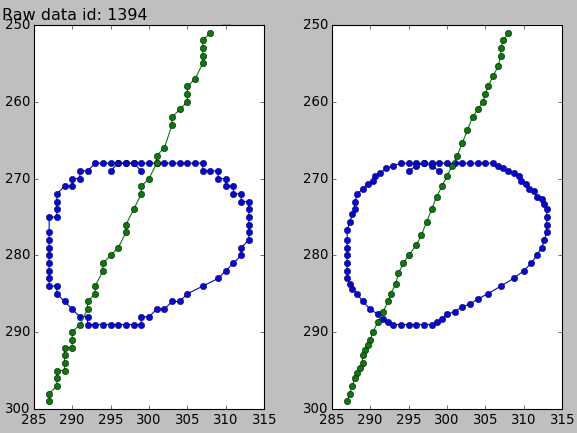
\includegraphics[width=6cm, keepaspectratio]{smooth-1-1-1.png}}
        \only<5>{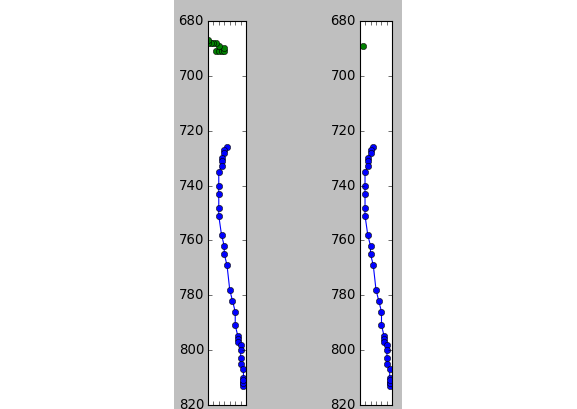
\includegraphics[width=6cm, keepaspectratio]{dot-reduction.png}}
        \only<6>{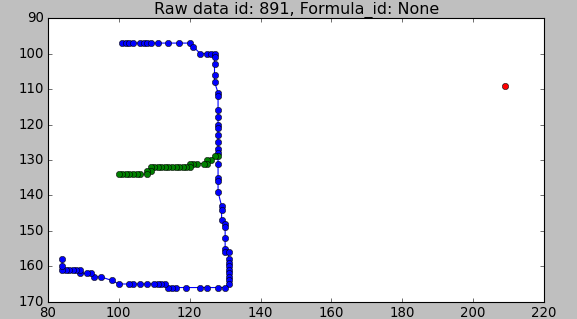
\includegraphics[width=6cm, keepaspectratio]{wildpoint-1.png}}
        \only<7>{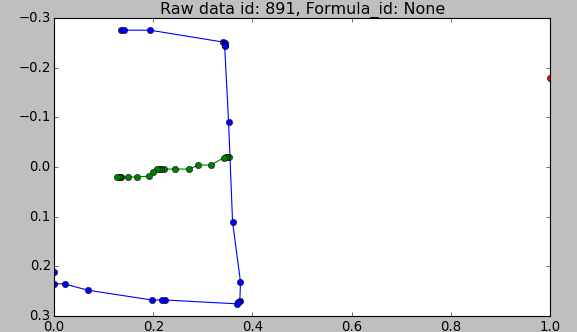
\includegraphics[width=6cm, keepaspectratio]{wildpoint-2.png}}
        \only<8>{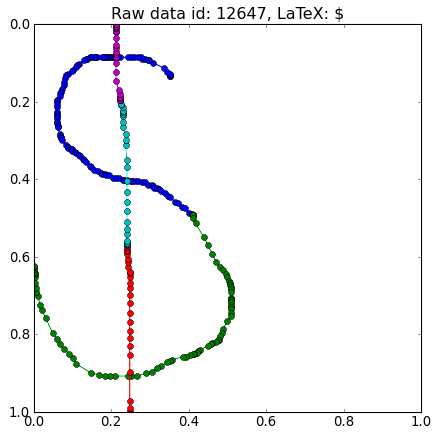
\includegraphics[width=6cm, keepaspectratio]{interrupted-stroke.png}}
    \end{column}
    \end{columns}


\end{frame}
\subsection{Features}
\begin{frame}{Features}
    \begin{itemize}
        \item Local
        \begin{itemize}
            \item Coordinates
            \item Speed
            \item Binary pen pressure
            \item Direction
            \item Curvature
            \item Bitmap-environment
            \item Hat-Feature
        \end{itemize}
        \item Global
        \begin{itemize}
            \item \# of points
            \item \# of strokes
            \item Center point
            \item Bitmap
            \item Bounding box (width, height, time)
            \item Re-curvature
            \item Ink
        \end{itemize}
    \end{itemize}
\end{frame}

\section{Neural Nets}
\subsection{Neural Net experiments}
\begin{frame}{Experiments}
    \textbf{Preprocessing:} Scaling, shifting and linear interpolation\\
    \textbf{Features:} Coordinates of 80 points (4 Lines with 20 points each)\\
    \textbf{Learning:} MLP, 300 epochs, LR of 0.1
    \begin{itemize}
        \item[] \textit{toplogy       \tabto{6cm} error in training time}
        \item 160:500:369             \tabto{6cm} 30.62 \% in \hphantom{0}9min 08s
        \item 160:500:500:369         \tabto{6cm} 27.73 \% in 11min 49s
        \item 160:500:500:500:369     \tabto{6cm} 34.79 \% in 14min 09s
        \item 160:500:500:500:500:369 \tabto{6cm} 33.61 \% in 14min 06s
    \end{itemize}
\end{frame}

\section{What will I do next?}
\subsection{What will I do next?}
\begin{frame}{What will I do next?}
    \begin{itemize}
        \item Evaluate preprocessing steps
        \item Try other features
        \item Try other topologies / trainings (e.g. pretraining, newbob)
    \end{itemize}
\end{frame}

% \subsection{Far future}
% \begin{frame}{What could be done?}
%     \begin{itemize}
%         \item Make use of audio data in a multimodal approach\\
%               e.g. $R$ and $\mathcal{R}$
%         \item Currently, the Lecture Translation system doesn't recognize math.\\
%               You get \enquote{integral of e raised to the power of x d x} instead
%               of $\int e^x \mathrm{d} x$.
%         \item Spoken math is ambigous: $\sqrt{a+b}$ vs. $\sqrt{a} + b$
%         \item The language model I create could help to find probable formulas
%         \item The platform could be used to get more input data of users
%     \end{itemize}
% \end{frame}

\section*{End}
\subsection{End}
\subsection{Sources}
\begin{frame}{Image Sources}
    \begin{itemize}
	\item \href{https://commons.wikimedia.org/wiki/File:Server-multiple.svg}{Server} by RRZEicons
    \item \href{https://commons.wikimedia.org/wiki/File:Computer-aj_aj_ashton_01.svg}{Desktop Computer} by Ed g2s,
          Ironbrother, Kierancassel and Msgj
    \item \href{https://commons.wikimedia.org/wiki/File:Server_by_mimooh.svg}{Server} by Mimooh
    \end{itemize}

    The presentation can be found at \url{http://tinyurl.com/write-math-short-presentation}
\end{frame}


\framedgraphic{Thanks for Your Attention!}{../images/xi.png}

\end{document}
